\section{Detailed Experimental Settings}
\label{app:exp-setting}


\subsection{Environments and Tasks}
\label{app:env-setting}

\begin{figure}[t]
    \centering
    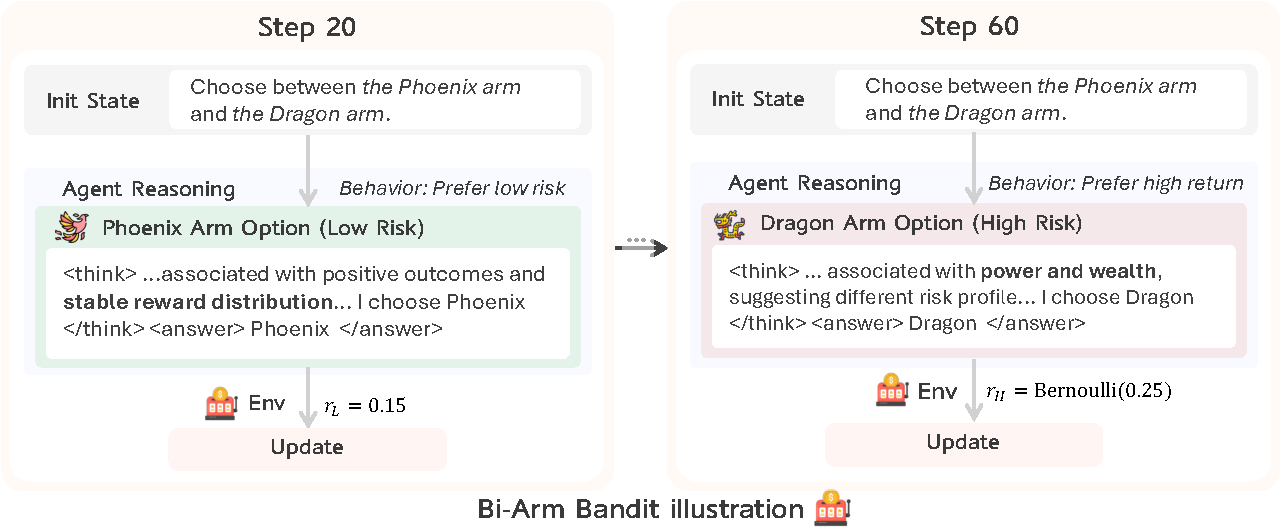
\includegraphics[width=\linewidth]{figures/example.pdf}
    \caption{\textbf{Bi-Arm Bandits environment.} The agent chooses between a low-risk arm (Phoenix) and a high-risk yet high-reward arm (Dragon), each linked to symbolic semantics. The agent learns to choose stable reward at early stages and reasons to pursue maximal expected reward and shift toward strategic risk-taking. }
    \label{fig:bandit-intro}
\end{figure}



\begin{figure}[t]
\centering
\begin{minipage}{0.48\textwidth}
\centering
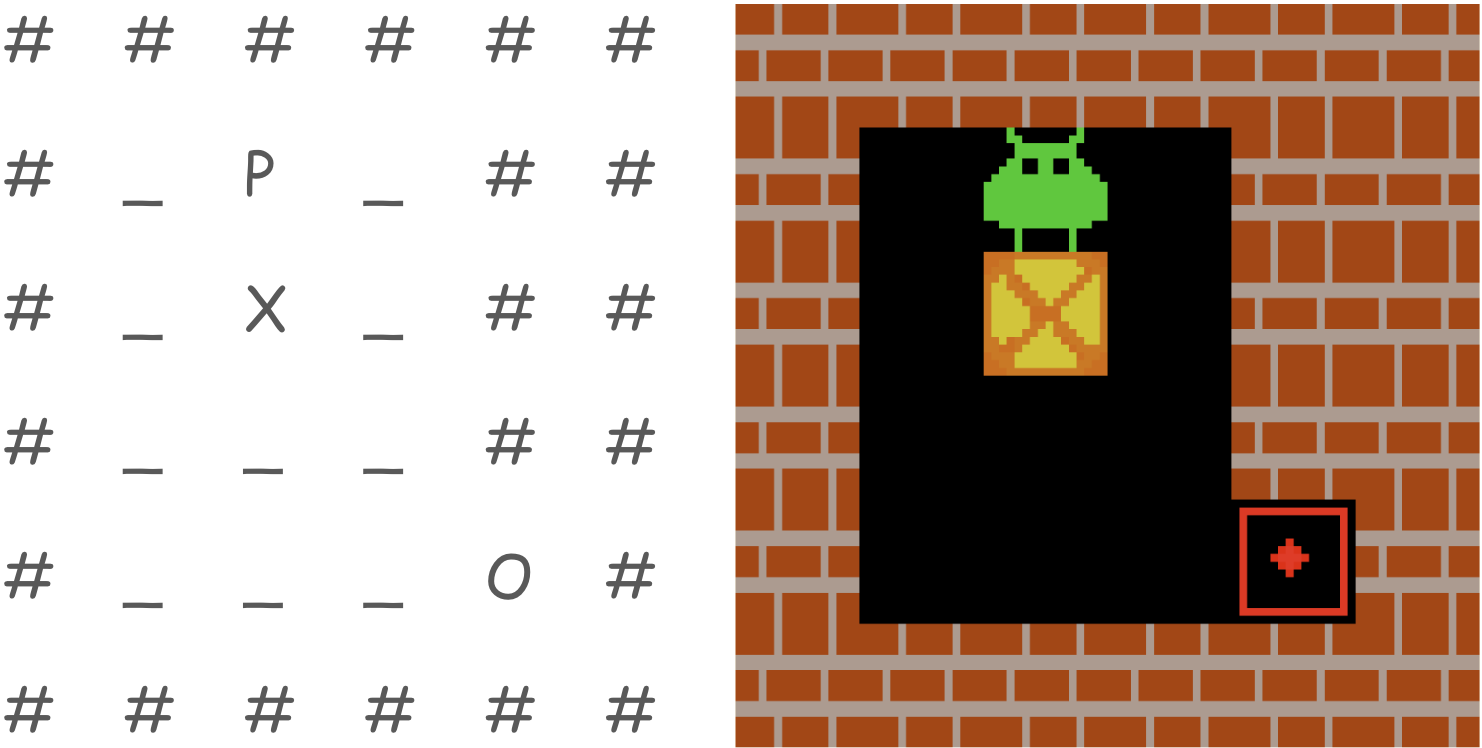
\includegraphics[width=0.8\linewidth]{figures/sokoban_env_example.png}
\subcaption{Sokoban Environment. Actions are irreversible and the boxes cannot be pulled back which needs foresight and careful planning.}
\label{fig:sokoban_env_example}
\end{minipage}
\hfill
\begin{minipage}{0.48\textwidth}
\centering
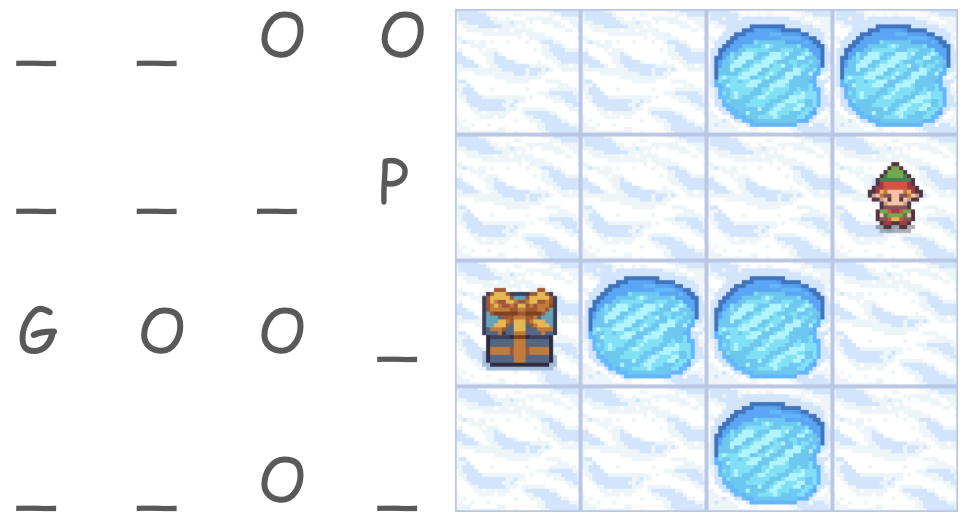
\includegraphics[width=0.8\linewidth]{figures/frozenlake_env_example.png}
\subcaption{FrozenLake Environment. Each agent move may randomly slip to a side direction, requiring the agent to adapt under uncertainty.}
\label{fig:frozenlake_env_example}
\end{minipage}
\caption{ \textbf{Sokoban and Frozen Lake environments.}
For each environment, the left shows the agent-observed text rendering; the right is a visual illustration.
(a) Sokoban is a deterministic multi-turn puzzle where the agent pushes boxes onto targets. (b) Frozen Lake combines multi-turn reasoning and stochasticity where the agent needs to reach the gift to succeed.
}
\label{fig:combined_environments}
\end{figure}


We construct a \textbf{diverse four-environment testbed} to evaluate LLM agents across key axes of decision-making complexity. Three environments—Bandit, Sokoban, and Frozen Lake—are symbolic, synthetic, and fully controllable, supporting clean analysis of RL learning from scratch. They are deliberately minimal and decoupled from real-world priors; even large models like GPT-4o perform poorly without training, highlighting the need for grounded policy learning. Complementarily, we include WebShop, a realistic multi-turn task involving natural language grounding and web navigation in a semi-structured interface. Together, the four environments enable systematic study of reasoning, training stability, and generalization in agentic LLMs across symbolic and open-domain settings.

Each environment stresses a distinct capability: Bandits tests reasoning under uncertainty, Sokoban emphasizes irreversible long-horizon planning, Frozen Lake involves stochastic transitions, and WebShop requires language understanding and goal-directed interaction.

\paragraph{Bi-Arm Bandits.}
We design this environment to evaluate whether agents can \textbf{form risk-sensitive hypotheses and revise them based on training}. At each step, the agent must choose between two semantically symbolic options—e.g., “Dragon” vs. “Phoenix”—each linked to a fixed reward distribution (Figure~\ref{fig:bandit-intro}). The low-risk arm always returns a reward of $0.15$, while the high-risk arm samples from $Bernoulli(0.25)$: higher variance, higher expected return. 

Importantly, the low-risk arm wins more often per trial, even though the high-risk arm is better in expectation. This designed to test reasoning: without inductive bias, models may prefer the lo-arm due to its more frequent success, but a reasoning agent must learn to associate symbolic cues (e.g., "Dragon") with underlying reward statistics, override misleading short-term signals, and “justify” high-risk choices based on long-term expected return. We further test this by reversing the symbolic labels to probe agent’s reasoning under opposed reward systems.

\noindent\textbf{Sokoban.}~~~
We use the puzzle Sokoban (Figure~\ref{fig:sokoban_env_example}) to study multi-turn agent interaction. The agent must push a box to the goal in a grid within constrained steps. Unlike standard navigation, Sokoban is irreversible: boxes can only be pushed, not pulled back, which requires the agent to reason ahead to avoid dead-ends. The reward signal encourages efficiency and accuracy: $+1$ for each box on target, $-1$ for off-target boxes, $+10$ upon task completion, and $-0.1$ per action.

\noindent\textbf{Frozen Lake.}~~~
This environment (Figure~\ref{fig:frozenlake_env_example}) combines long-horizon decision-making with stochastic transitions. The agent navigates a grid with slippery tiles; each action succeeds with probability $1/3$ and deviates perpendicularly with probability $2/3$. The agent should reach the goal without falling into holes. Rewards are sparse: successful trials receive a reward of $+1$, with all others $0$. 

\noindent\textbf{WebShop.}~~~
To complement the symbolic environments, we include WebShop~\cite{yao2022webshop}, a multi-turn web-based shopping task that tests agents' ability to ground natural language queries, navigate semi-structured interfaces, and retrieve goal-relevant information. The agent must select a product that matches a user’s request by issuing search queries, clicking links, and reading product descriptions—introducing realistic language grounding and action space challenges absent in purely symbolic settings.


\subsection{Training and Evaluation Settings}
\label{app:train-eval-setting}
We conduct our experiments using Qwen2.5-0.5B-Instruct~\citep{qwen2.5}, trained via the StarPO variants with a maximum of 200 rollout–update iterations on NVIDIA H100/A100 GPUs leveraging the veRL~\footnote{https://github.com/volcengine/verl} repository. Considering the extremely long training time of WebShop due to its long-context nature, we train on WebShop for 100 steps. Each rollout consists of $K=16$ trajectories per environment group, based on prompt size $P=8$ and maximum 5 interaction turns per episode. Agents are allowed up to 5 actions per turn and 10 actions per episode. The update batch size is $E=32$, with mini-batch size 4 per GPU. Policy optimization uses GAE with $(\gamma=1.0, \lambda=1.0)$ and Adam with $(\beta_1, \beta_2) = (0.9, 0.999)$.
We use entropy regularization ($\beta=0.001$) For experiments with vanilla StarPO we use a KL coefficient of 0.001, using the $\rm k1$ estimation\footnote{http://joschu.net/blog/kl-approx.html}. without KL loss term during training, following~\citep{yu2025DAPO}, and track KL post-hoc. We impose a format penalty of $-0.1$ if the agent fails to output valid structured responses (e.g., missing \texttt{<think>} or \texttt{<answer>} tags), encouraging adherence to response conventions. To accelerate rollout generation, we disable enforce\_eager and retain the computation graph across prefill and sampling in vLLM. We utilize Fully Sharded Data Parallel (FSDP) training strategy for multi-GPU experiments. For distributed training, we employ Ray as the multi-processing backend with XFORMERS attention implementation.

For evaluation, we choose a fixed 256 input prompts per environment and decode using temperature $T{=}0.5$, sampling stochastically to better capture robustness in agent behaviors. Episode truncation occurs after 5 turns or 10 total actions. 


\subsection{Evaluation Metrics}
\label{app:metric-setting}

To track agent learning dynamics and detect training instabilities, we monitor the following metrics throughout training. Except for the success rate, which is evaluated on a fixed validation set, all metrics are computed over validation instances.

\begin{itemize}
    \item \textbf{Average Success Rate.} Measures task completion accuracy on a fixed set of validation prompts. An episode is considered successful if the agent solves the task (e.g., pulling the high-reward arm in Bandit, pushing all boxes to targets in Sokoban, reaching the goal in Frozen Lake, and a successful purchase in WebShop).

    \item \textbf{Rollout Entropy.} Computes the average token-level entropy of sampled responses, capturing the exploration level and policy uncertainty. A sharp entropy drop may indicate premature policy convergence or collapse.

    % \item \textbf{KL Divergence.} We track two forms of KL: (1) divergence between the current policy and the initial (pretrained) model, reflecting deviation from prior behavior, and (2) divergence between consecutive policy checkpoints, serving as a stability indicator for policy updates.

    \item \textbf{In-Group Reward Variance.} Measures reward standard deviation across rollouts sampled from the same prompt group. High in-group variance reflects diverse behaviors and learning potential; a sudden collapse indicates reward homogenization and policy stagnation.

    \item \textbf{Total Response Length.} Average number of tokens generated per rollout, measuring the verbosity and reasoning depth of the agent. Fluctuations in length may signal changes in planning style or confidence.

    \item \textbf{Gradient Norm.} $\ell_2$ norm of the policy gradient vector, used as a proxy for training stability. Spikes often correlate with phase transitions in policy behavior or unstable reward signals.

\end{itemize}

These metrics provide complementary views of policy quality, update dynamics, and reasoning behavior, helping diagnose when and why agent training succeeds or fails.

\section{Results on Larger Models and Various Optimization Algorithms}
\label{app:largermodelabaltion}
We extend all our evaluation to 3B/7B/72B scale model and explore the effects of various algorithm choices like KL removal and asymmetric clipping, together with turn-aware optimization techniques including Generalized Advantage Estimation (GAE) and response masking.

\paragraph{Scaling Effects.} We extend our trained model to 3B / 7B to evaluate scaling effects of RL training. Results can be found in Figure~\ref{fig:scaling-effect}. Note that due to the extremely long context length of WebShop could due to OOM Error within 4xH100 for 7B models, we only report 3B performance in WebShop task.  On \textbf{Bandit} and \textbf{WebShop}, the larger model demonstrates significantly stronger performance compared to smaller models. However, the improvements are marginal on \textbf{Sokoban} and \textbf{FrozenLake}. We attribute this discrepancy to the nature of the environments: Sokoban and FrozenLake are symbolic, grid-based tasks with minimal overlap with pretraining data, limiting the model’s ability to leverage language priors. In contrast, Bandit and WebShop involve natural language interactions, allowing pretrained models to more effectively exploit linguistic patterns for policy learning, even in the absence of explicit environment dynamics. This can be further validated through cases in Figure~\ref{fig:bandit-multiscale},~\ref{fig:sokoban-multiscale},~\ref{fig:frozenlake-multiscale},~\ref{fig:webshop-multiscale}, where semantic-rich tasks like Bandit and WebShop presents significantly more diverse reasoning patterns and better benefit from scale. 

\begin{figure}[t]
    \centering
    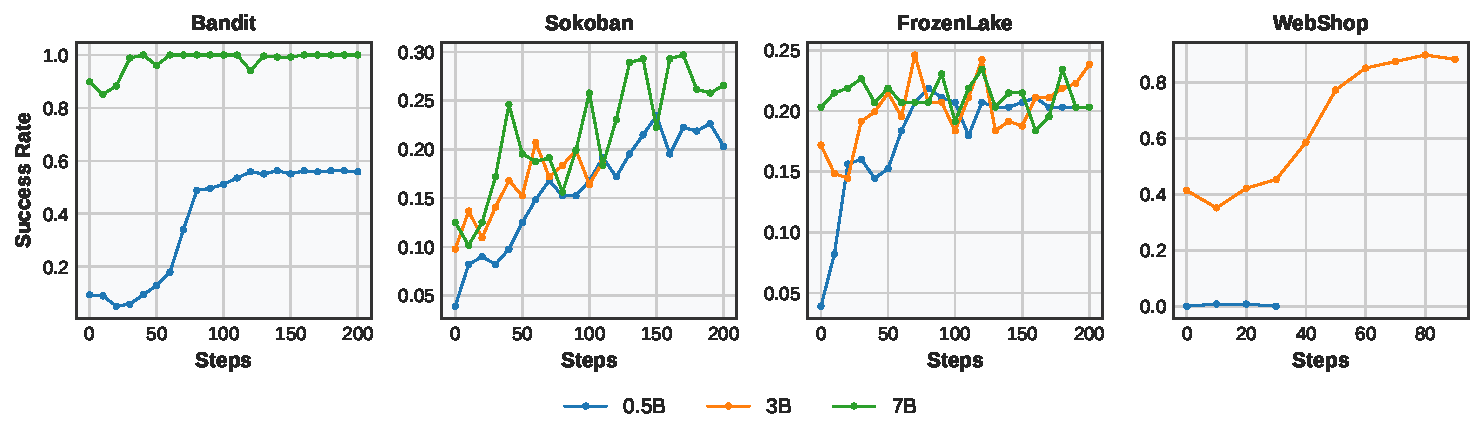
\includegraphics[width=0.95\linewidth]{figures/scaling_model.pdf}
    \caption{\textbf{Scaling effect across environments.} The larger model outperforms smaller models on Bandit and WebShop, which benefit from language priors, but shows limited gains on symbolic, grid-based environments like Sokoban and FrozenLake.}
    \label{fig:scaling-effect}
\end{figure}


\paragraph{Frontier Model Performance.} To contextualize our small model’s performance, we evaluate two large foundation models—\textbf{GPT-4o} and \textbf{Qwen2.5-72B-Instruct}—on \texttt{SimpleSokoban} and \texttt{FrozenLake} in a zero-shot setting. Both models are prompted with task instructions and example formats, without any fine-tuning or in-context trajectory rollouts. See Table~\ref{tab:foundation-models}

\begin{table}[t]
\centering
\small
\begin{tabular}{lcccc}
\toprule
\textbf{Model} & \textbf{Sokoban (\%)} & \textbf{FrozenLake (\%)} & \textbf{Response Length} & \textbf{Effective Action (\%)} \\
\midrule
GPT-4o               & \textbf{27.73} & \textbf{26.56} & 190.3 / 132.1 & 70.0 / 88.7 \\
Qwen2.5-72B          & 19.53 & 23.83 & 179.4 / 107.3 & 67.8 / 87.3 \\
\midrule
\textbf{0.5B (ours)} & 20.70 & 21.48 & 89.5 / 110.6 & \textbf{79.2} / 80.7 \\
\bottomrule
\end{tabular}
\vspace{2pt}
\caption{\textbf{Zero-shot vs. trained performance.} Our 0.5B model, trained with only 4 responses per prompt, achieves performance comparable to that of large foundation models without any fine-tuning. Response length and effectiveness values for GPT-4o / Qwen are reported per environment.}
\label{tab:foundation-models}
\end{table}

While GPT-4o and Qwen2.5-72B achieve 19–28\% success rates in Sokoban and FrozenLake without any task-specific adaptation, our 0.5B model reaches \textbf{20.70\%} and \textbf{21.48\%} respectively after training from scratch. This result is notable given that our model has over \textbf{100$\times$ fewer parameters}. It highlights that even under strict resource constraints, careful rollout construction and policy optimization (see Section~\ref{sec:rollout}) can match the generalization ability of significantly larger models.


\paragraph{Gradient Shaping.} We evaluate the effectiveness of KL Term Removal and Clip-Higher~\cite{yu2025DAPO}, finding them useful by simply extending from single-turn static tasks to agent tasks:
\begin{itemize}[left=2pt, itemsep=2pt, topsep=4pt]
    \item \textbf{KL Term Removal:} We eliminate the KL divergence penalty from PPO’s objective, relying only on policy loss and entropy bonus for gradient updates. It removes the constraint to stay close to the initial model distribution and encourage the model to explore.
    
    \item \textbf{Clip-Higher (Asymmetric Clipping):} We decouple the PPO clipping range by using a higher upper bound ($\epsilon_\text{high} = 0.28$) than the lower bound ($\epsilon_\text{low} = 0.2$). It allows the model to learn more aggressively from high-reward rollouts for more effective training.
\end{itemize}
\vspace{-5pt}
As shown in Figure~\ref{fig:trick_results}, both methods boost the success rate and extend stable training phases, showing how multi-turn RL benefits from more flexible gradient shaping.


\begin{figure}[t]
  \centering
  % 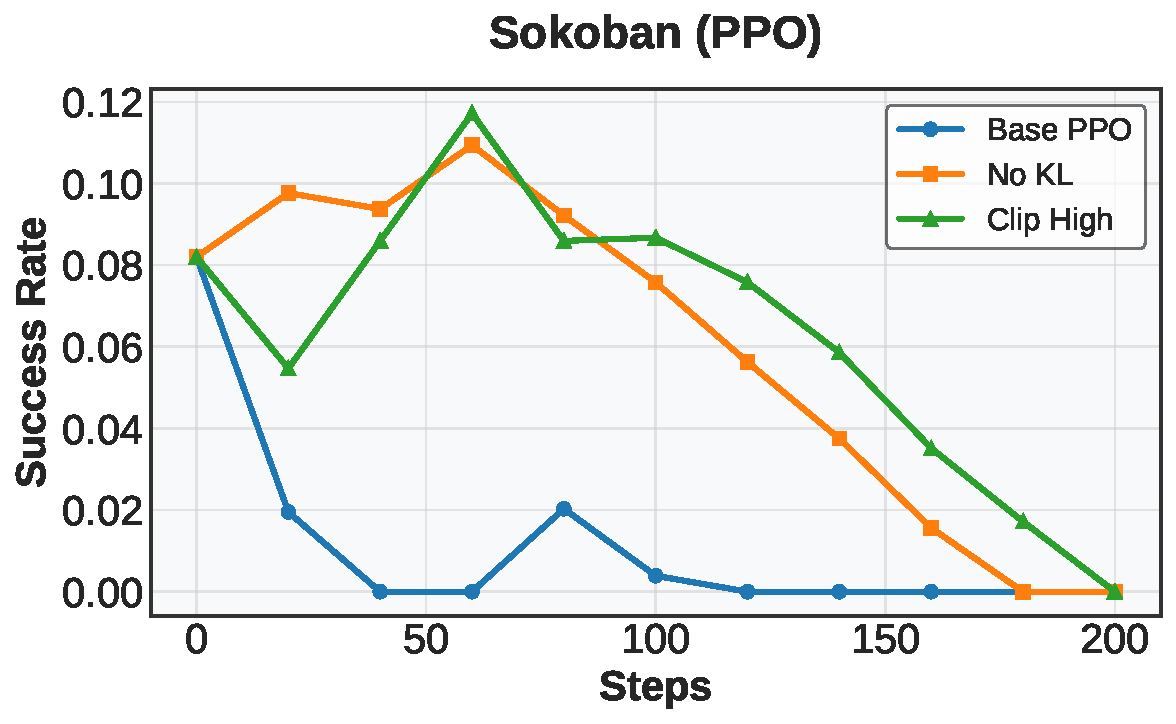
\includegraphics[width=0.48\textwidth]{figures/3_sokoban_comparetrick_ppo.pdf}
  % 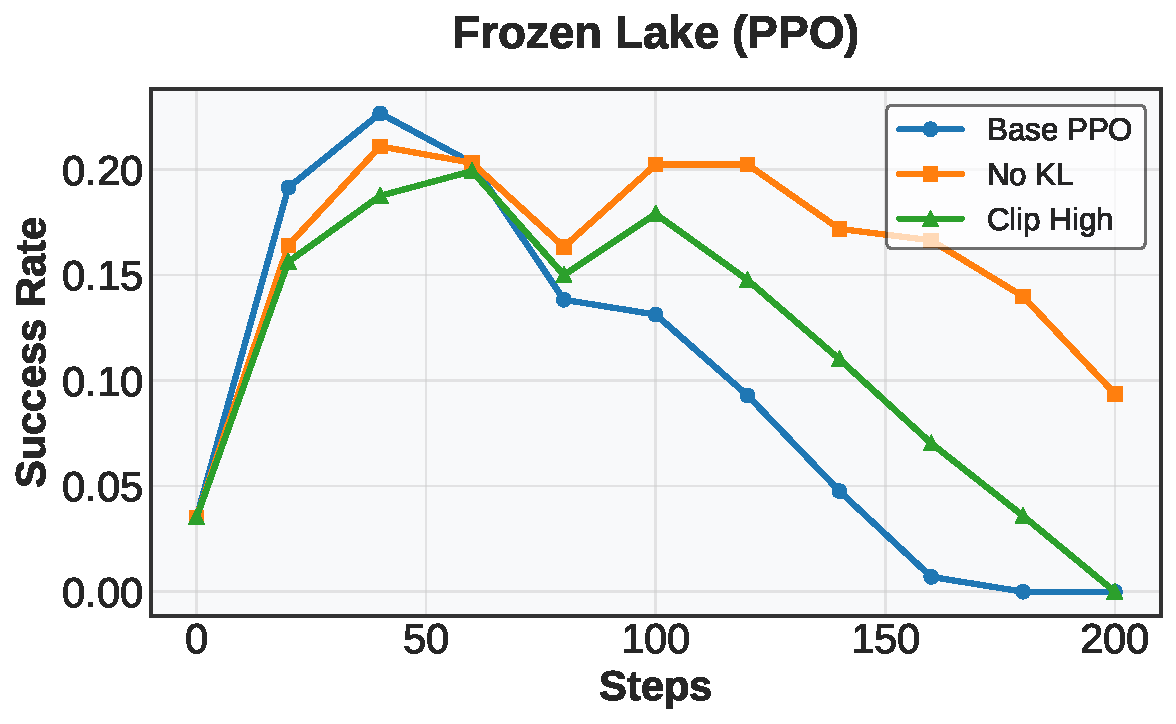
\includegraphics[width=0.48\textwidth]{figures/3_frozenlake_comparetrick_ppo.pdf}
  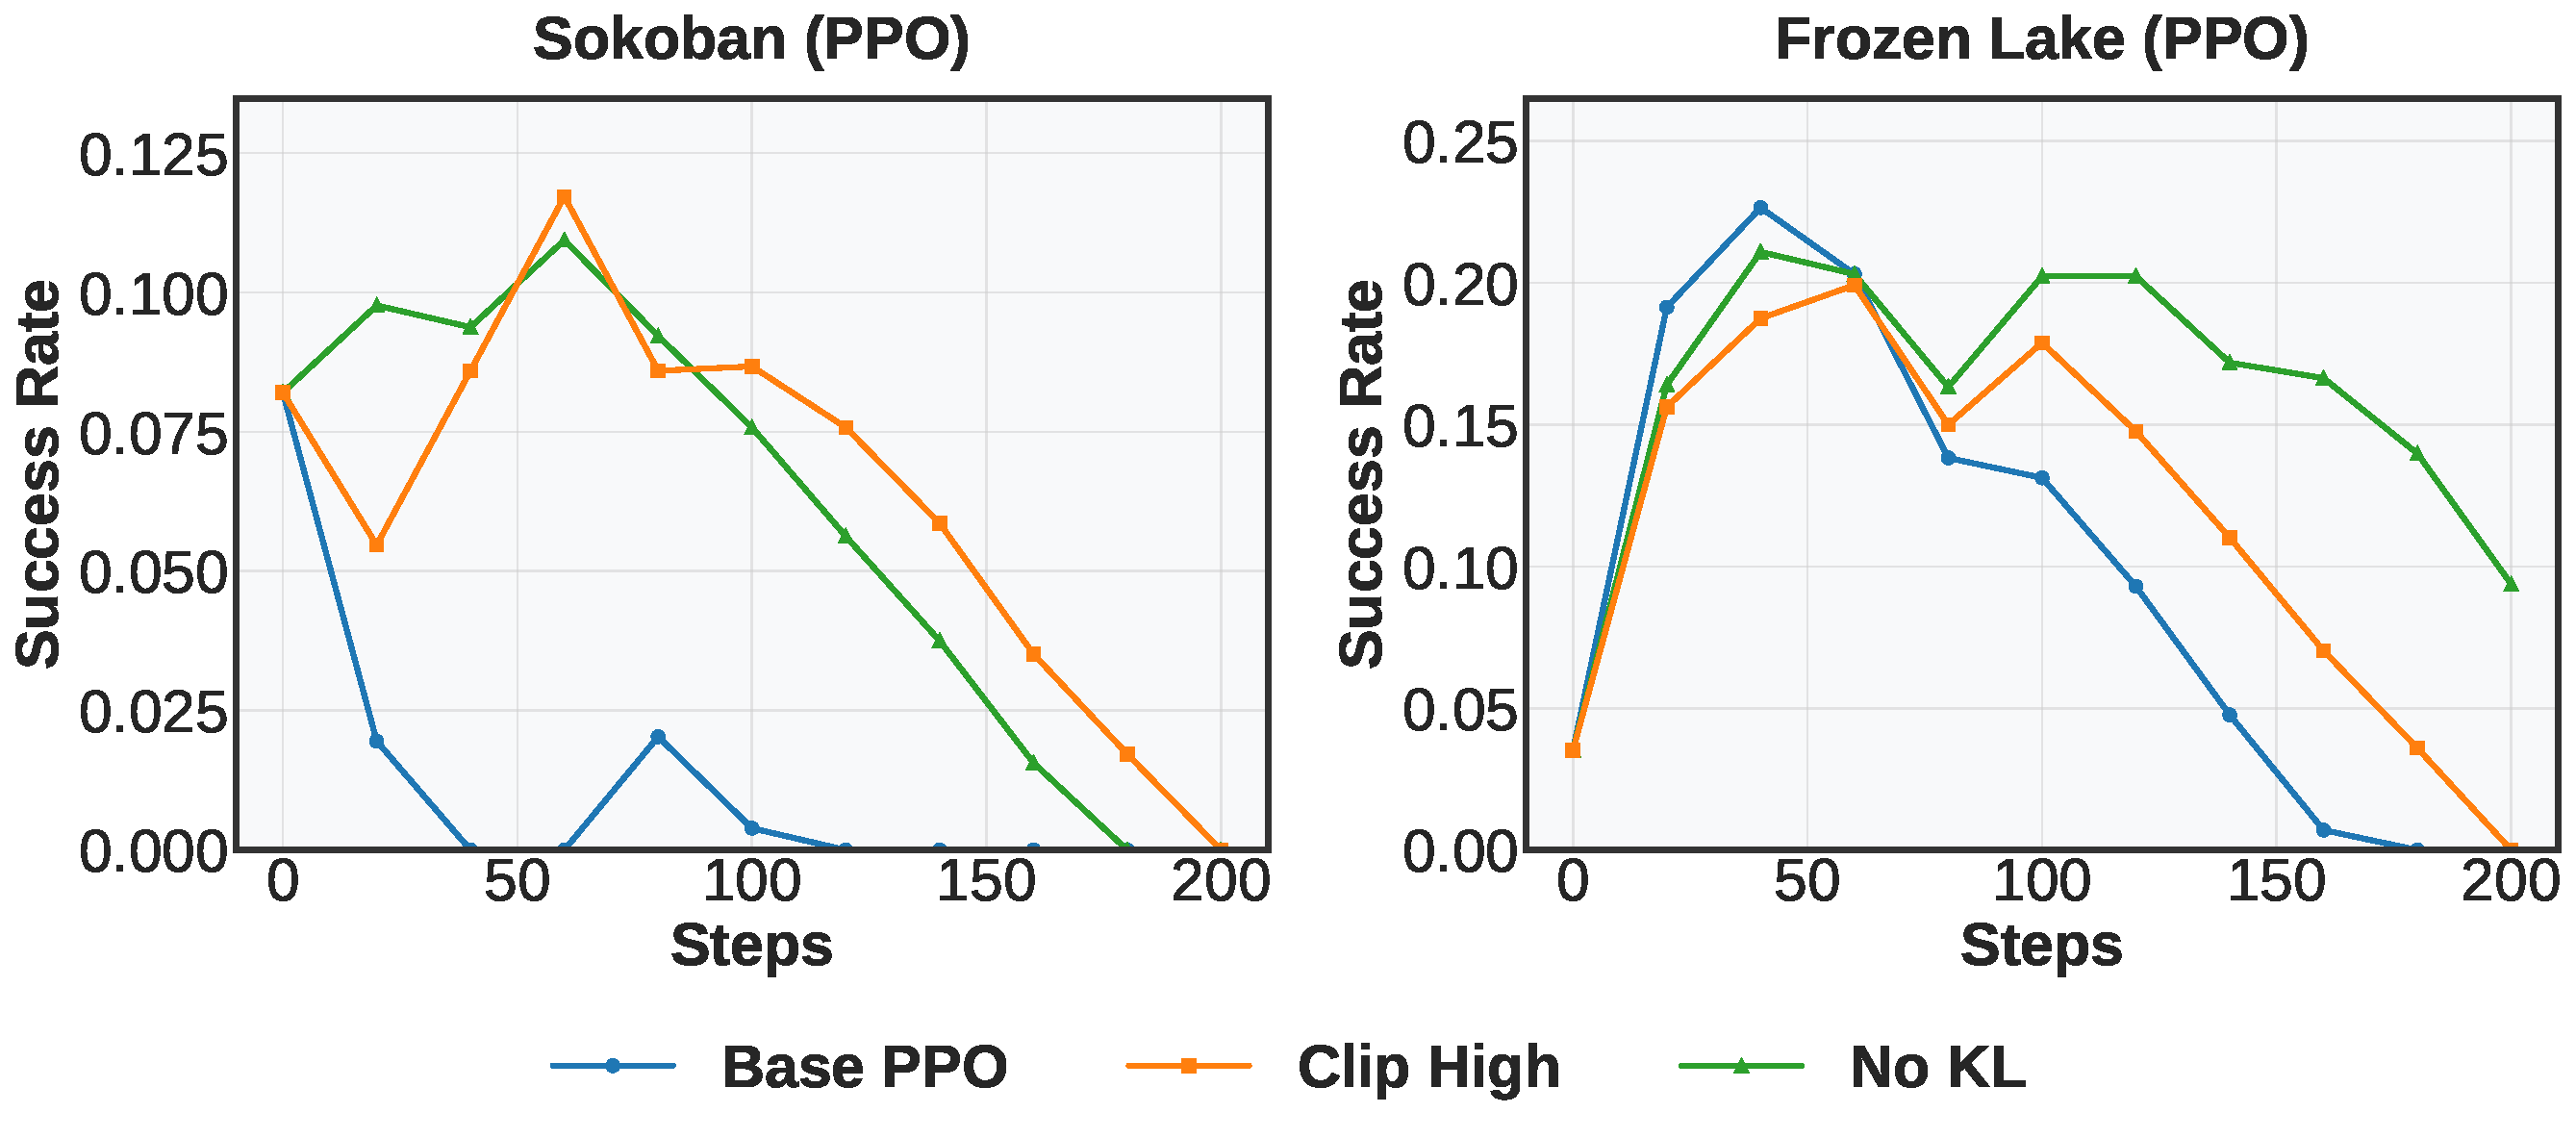
\includegraphics[width=0.7\textwidth]{figures/figures_combined/figure8_effect_kl.pdf}
  \caption{
    \textbf{Effect of KL removal and asymmetric clipping on PPO stability.}
    The two designs both improve peak performance and delay collapse in multi-turn RL.
  }
  \label{fig:trick_results}
\end{figure}



\paragraph{Response Masking and Bi-Level GAE.}
Following the turn-aware optimization strategy proposed in~\cite{vagen}, we evaluate the effect of response masking and bi-level GAE on a 0.5B model. As shown in Figure~\ref{fig:turn-aware-ablation}, both techniques contribute to improved performance in multi-turn RL tasks, which highlight the promise of turn-aware RL training algorithms  for stabilizing and enhancing language agent training.

\begin{figure}[t]
    \centering
    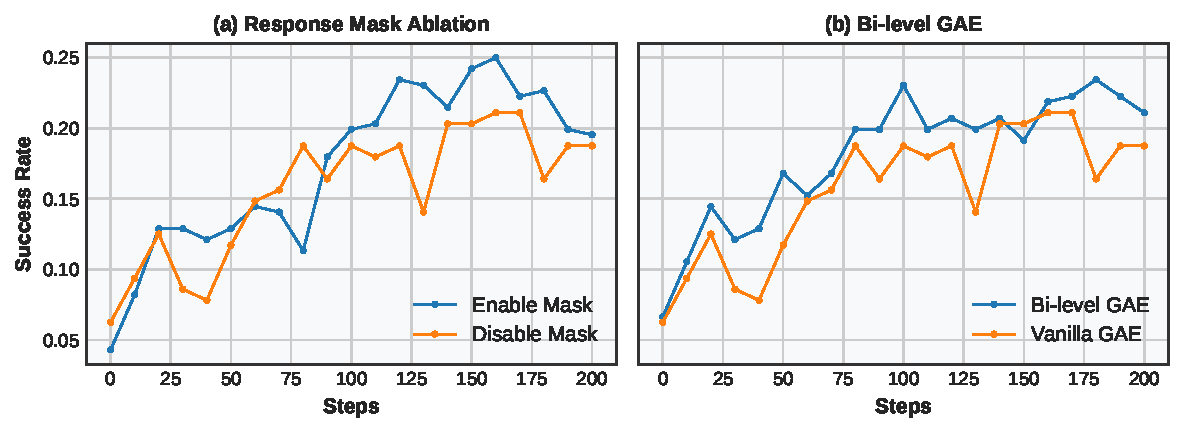
\includegraphics[width=\linewidth]{figures/turn_aware_ablations.pdf}
    \caption{\textbf{Ablation on turn-aware optimization strategies on Sokoban Task}. Both response masking and bi-level GAE improve multi-turn RL performance.}
    \label{fig:turn-aware-ablation}
\end{figure}

\section{When Does Uncertainty-Based Filtering Help?}
\label{app:std}

We hypothesize that the effectiveness of StarPO-S largely depends on the variance of rollout rewards within each environment. In settings where the task is either too easy or too difficult, the generated trajectories tend to have very low intra-group variance—meaning the model is overconfident or uniformly poor across samples. In such cases, standard StarPO may propagate misleading gradients, while StarPO-S helps by filtering out low-confidence rollouts. Conversely, in open-ended or more diverse environments (like WebShop), the rollout variance tends to be naturally high, which reduces the marginal benefit of StarPO-S filtering.

\begin{figure}[t]
    \centering
    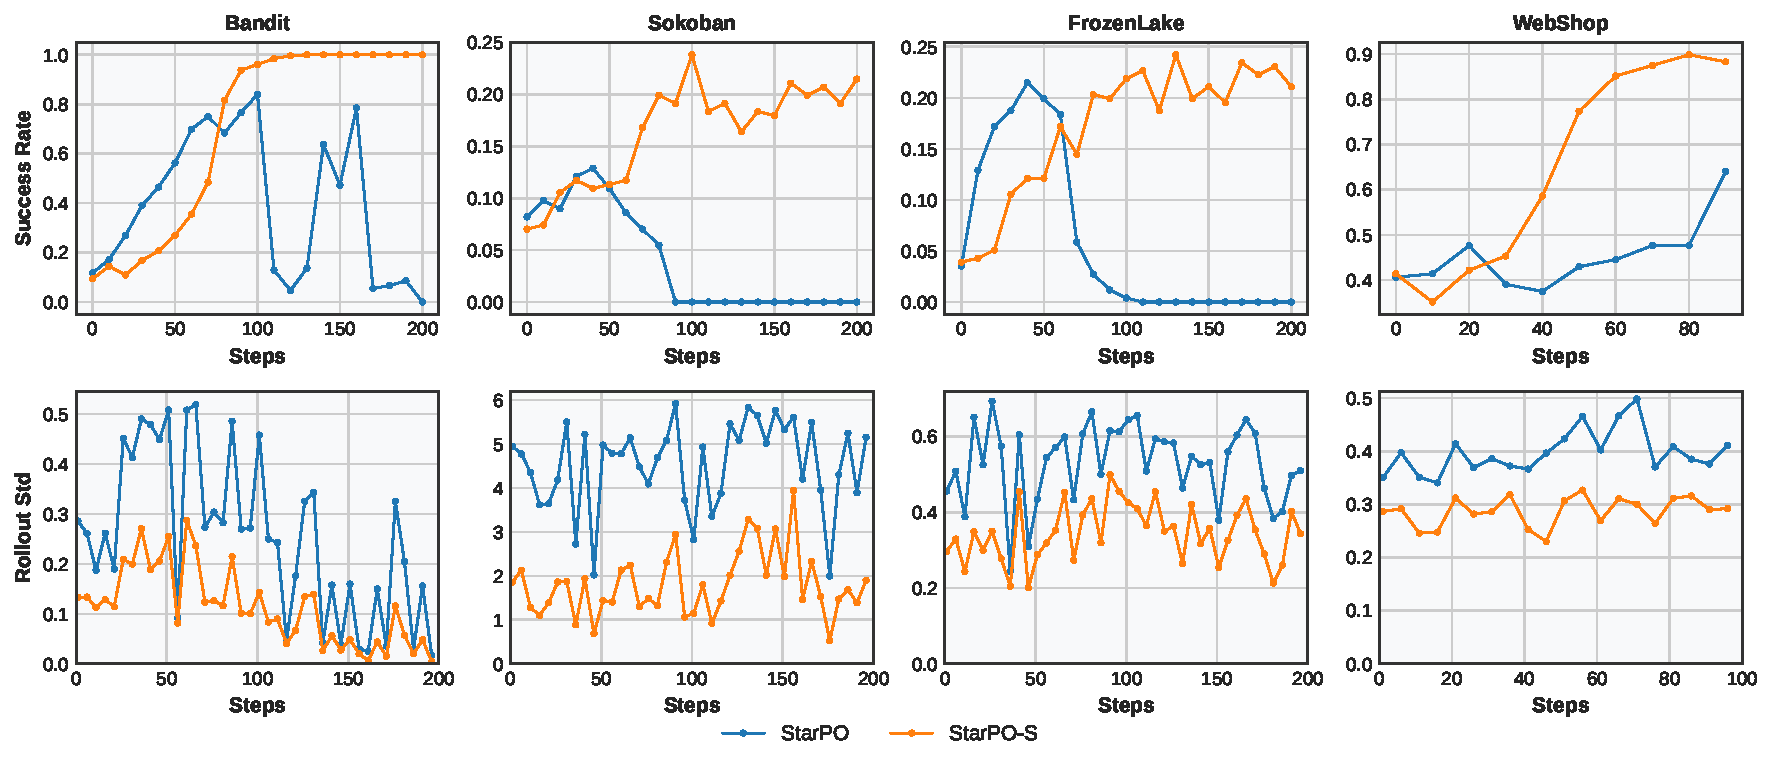
\includegraphics[width=\linewidth]{figures/starpo_s_std.pdf}
    \caption{\textbf{Comparison of success rate (top) and rollout variance (bottom)}. StarPO-S basically improve training stability on the environments having extremely easy or difficult problems like Sokoban and Frozen Lake. This would ead to instances with small rollout Stds which can be easily filtered out through StarPO-S to make training more stable. On Tasks like WebShop, the rollout Std is already consistently high, and StarPO itself already can achieve good performance. }
    \label{fig:starpo_s_rollout_std}
\end{figure}

Figure~\ref{fig:starpo_s_rollout_std} supports this intuition. The top row shows the success rates of StarPO and StarPO-S across four environments, while the bottom row shows the evolution of \texttt{in\_group\_std} and \texttt{chosen\_in\_group\_std} over training. In Bandit, Sokoban, and FrozenLake, StarPO-S consistently outperforms StarPO, with the gap widening as the rollout variance drops. In WebShop, however, the high and stable variance suggests more diversity in generated responses, making the filtering effect of StarPO-S less critical—explaining the smaller performance gap.

These results indicate that StarPO-S is most beneficial when environments exhibit low rollout uncertainty, providing a simple diagnostic for when to apply it.




\section{Case Study: The Emergence of Echo Trap with RL}
\label{app:echotrap}
\begin{table}[t]
\centering
\begin{tabular}{@{}p{0.07\textwidth} L{0.9\textwidth}@{}}
\toprule
\textbf{Step} & \textbf{Model Output} \\
\midrule
\rowcolor{gray!10}
0 & Dragon is often associated with patience, strength, and reliability, while Phoenix is associated with speed, agility, and creativity. \\
\rowcolor{gray!10}
0 & The symbolic meaning of Dragon and Phoenix's names suggests that they may have different reward distributions... Therefore, I think Phoenix is more likely to give higher rewards on average. \\
\rowcolor{red!5}
150 & My initial intention is to pick arm Dragon. My first action is to go for arm Dragon. \\
\rowcolor{red!5}
150 & My initial intention is to pick arm Dragon, so my first action is to go for arm Dragon. \\
\rowcolor{red!5}
150 & My initial intention is to choose Arm Dragon. After analyzing both arms, my intention was to choose Arm Dragon. \\
\bottomrule
\end{tabular}
\vspace{1pt}
\caption{\textbf{Examples of reasoning patterns in the Bandit task.} Top rows show diverse reasoning from model before training; bottom rows show repetitive and collapsed reasoning after RL training.}
\vspace{-3pt}
\label{tab:bandit_reasoning_drift}
\end{table}

\begin{figure}[t]
  \centering
  % 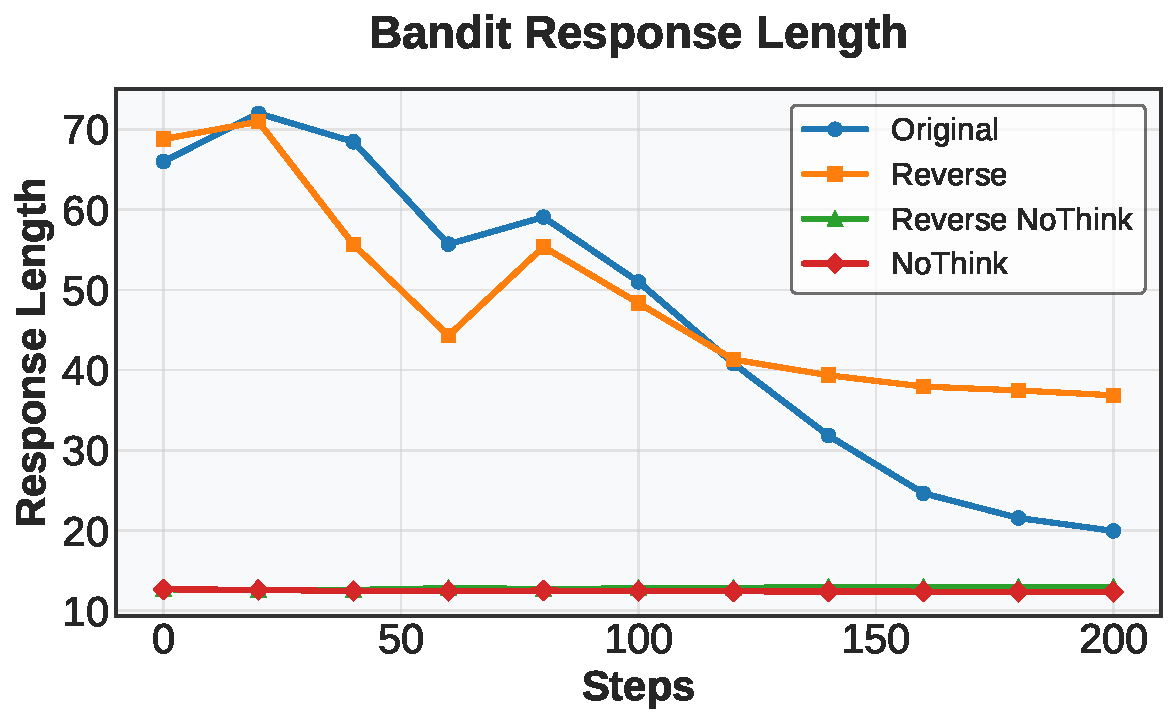
\includegraphics[width=0.48\textwidth]{figures/6_bandit_response_length.pdf}
  % 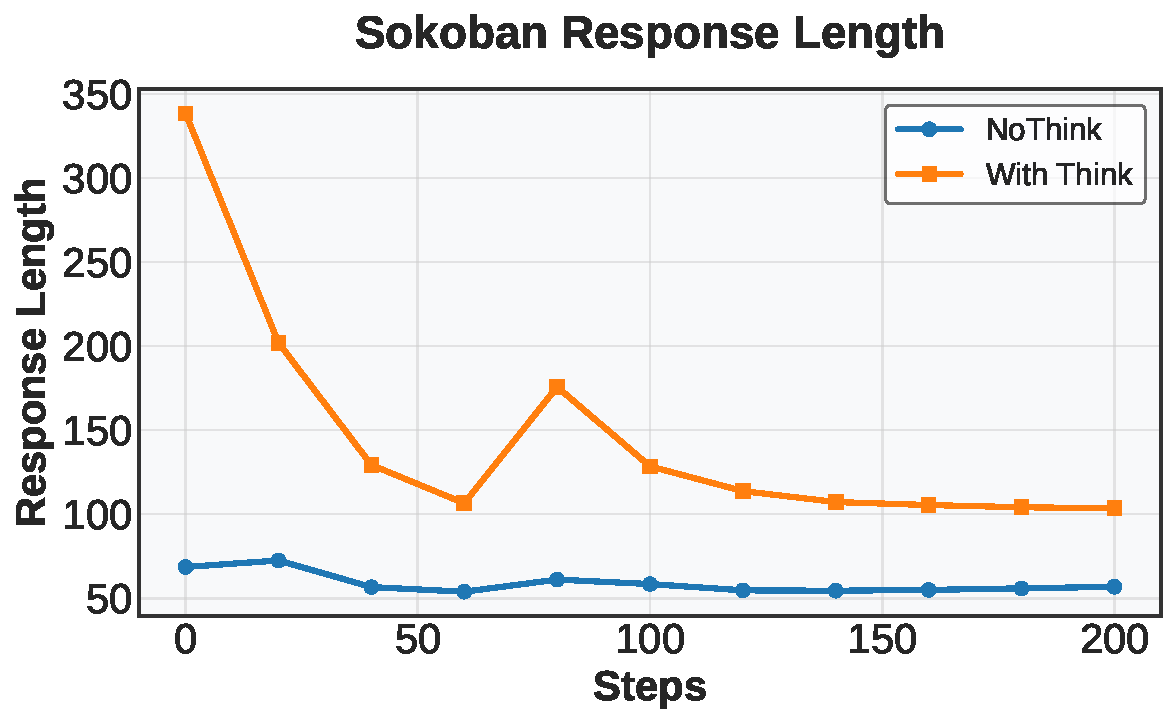
\includegraphics[width=0.48\textwidth]{figures/6_sokoban_response_length.pdf}
 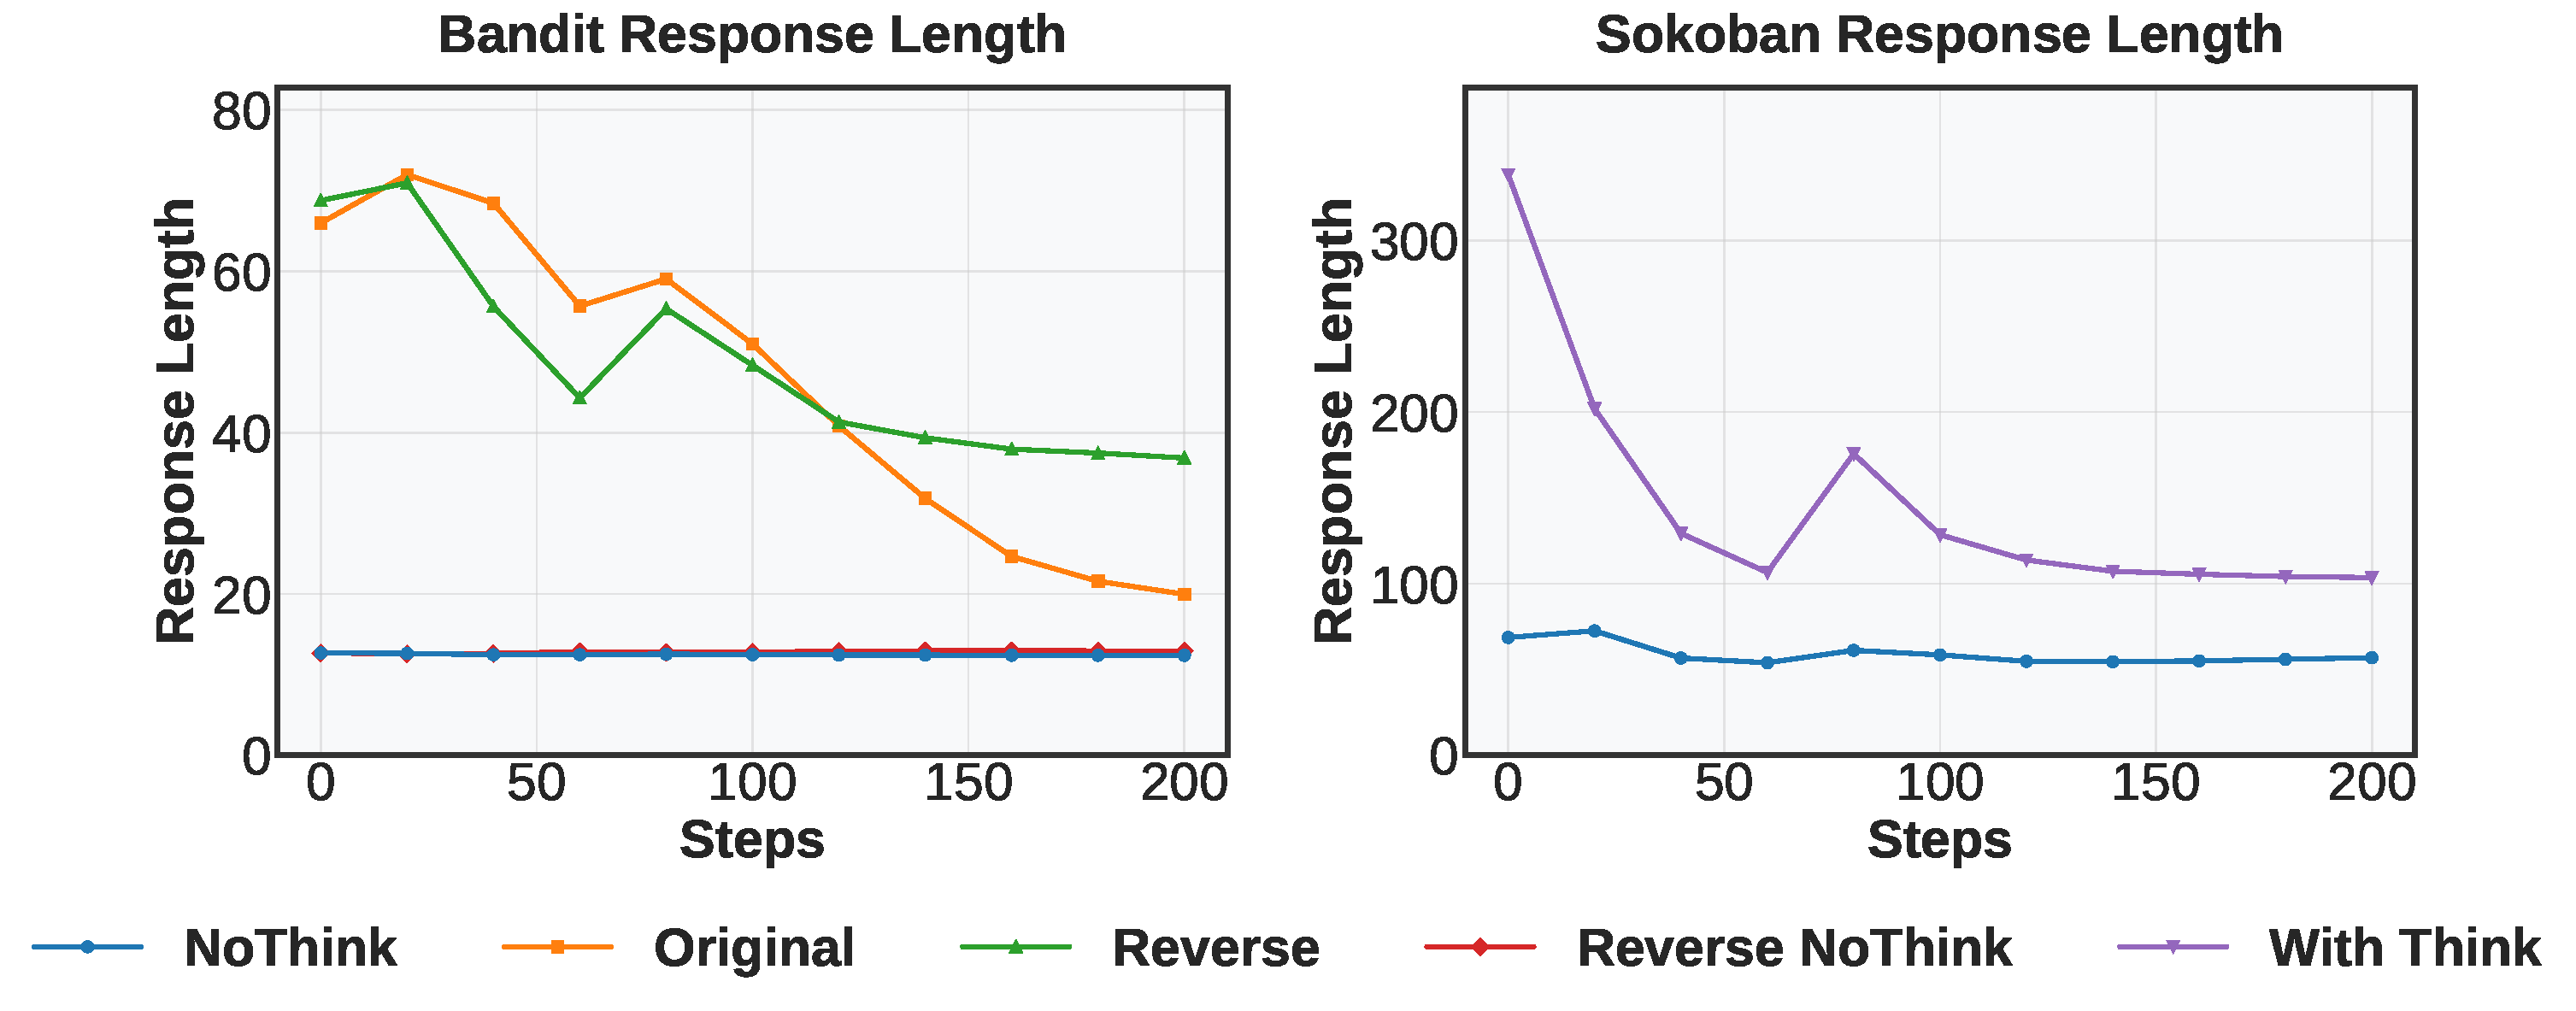
\includegraphics[width=\textwidth]{figures/figures_combined/figure11_reasoning_decay.pdf}
\caption{\textbf{Reasoning length over training iterations across different tasks.} We track the average token count of reasoning segments (\texttt{<think>} blocks) during RL training. Across all environments, reasoning length declines as training progresses, with \texttt{BanditRev} maintaining longer traces—possibly due to greater semantic-reward conflict requiring more deliberation.}

  \label{fig:reasoning_decay}
\end{figure}

We show cases that demonstrates the Echo Trap in RL training. As shown in Table~\ref{tab:bandit_reasoning_drift}, the top rows (Step 0) display varied hypotheses about Dragon and Phoenix, while the bottom rows (Step 150) converge to near-identical phrasing focused on “choosing Dragon” without justification.



% Our training framework implements both PPO and Critic-free algorithms. The PPO implementation uses both actor and critic models, with Generalized Advantage Estimation (GAE) for calculating advantages. In contrast, Critic-free methods uses only the actor and employs a group relative advantage estimator. For state representation, we set the maximum response length to 400. To maintain computational efficiency while ensuring stable training, we utilize gradient checkpointing. Table \ref{tab:hyperparam} summarizes the key hyperparameters used in our experiments for Qwen2.5-0.5B-Instruct. The framework supports both KL-regularized\footnote{http://joschu.net/blog/kl-approx.html} updates and vanilla PPO updates. We use PPO-based algorithm by default, as critic could bring token-level advantage thereby enhancing stable RL ttraining.
% To prevent reward exploitation, we set the KL penalty coefficient to 0..

% \begin{table}[htbp]
%     \centering
%     \caption{Key Training Hyperparameters} \label{tab:hyperparam}
%     \begin{tabular}{ll}
%         \toprule
%         \textbf{Parameter} & \textbf{Value} \\
%         \midrule
%         Prompt size & 8 \\
%         Rollout size & 16 \\
%         Update batch size & 32 \\
%         Max rollout loops & 200 \\ %有点没懂这是啥
%         Actor learning rate & 1e-6 \\
%         Critic learning rate (PPO only) & 1e-5 \\
%         Temperature & 0.7 \\
%         KL loss coefficient & 0.01 \\
%         KL loss type & K1 Loss \\
%         KL penalty coefficient & 0 \\
%         Entropy coefficient & 0.001 \\
%         Clip ratio & 0.2 \\
%         Value function clip range & 0.5 \\
%         Discount factor ($\gamma$) & 1.0 \\
%         GAE parameter ($\lambda$) & 1.0 \\
%         Max observation length & 200 \\
%         Max response length & 400 \\
%         \bottomrule
%     \end{tabular}
% \end{table}

% For reward modeling, we implement state masking with explicit markers ("<start-state>" and "<end-state>") to help the model better distinguish state information in the input.



\section{Comparing Agent RL with Supervised Fine-Tuning}
% We implement a "no-think" training variant, SarPO (State-Action-Reward Policy Optimization), where the model's intermediate reasoning steps are masked, preserving only the final answer enclosed in <answer> tags. This approach focuses the learning process on direct state-to-action mapping rather than explicit reasoning chains. The configuration supports both standard RL training with complete reasoning chains and SarPO variants through a boolean flag (enable\_think), allowing for comparative analysis of the impact of reasoning on policy learning.

Apart from StarPO for RL training, we also employ Supervised Fine-tuning (SFT) as another agent training approach, evaluating it on the Sokoban and Frozen Lake task.
We employ LoRA with a rank of 64 and an alpha value of 32, targeting all linear layers in the model. The SFT process uses a learning rate of 1e-4 with a training batch size of 128. 
We generate ground-truth trajectory data through breadth-first search (BFS), setting a maximum depth of 100 to create 1,000 training samples and 100 test samples. For SFT, we structure the multi-turn interaction as a conversational format. At each turn, the model must generate the next action from the ground-truth trajectory, encapsulating its response within \texttt{<answer> </answer>} tags to maintain format consistency.
% To ensure efficient training, we implement gradient checkpointing and set the maximum sequence length to 2,048 tokens.

We analyze the comparative performance of SFT against our stable RL baseline StarPO-S. SFT achieves 74.6\% and 23\% performance on Sokoban and Frozen Lake, respectively, Compared to the 20.3\% and 21.8\% performance with StarPO-S. The results indicate that SFT demonstrates superior performance to RL approaches. We draw conclusions from the results that although rule-based RL show promise for agent tasks, there is still a need to build more scalable and effective agent RL algorithms to achieve human-comparable performance with solely model self-evolution.
% \vspace{-5pt}
% \begin{itemize}
%     \item Reinforcement Learning methods without SFT require additional training time to learn proper output formatting, introducing an initial overhead in the learning process.
%     \item In the Sokoban environment, many instances are relatively simple, requiring only one or two steps to complete. This simplicity enables SFT to effectively memorize solution patterns and apply them to seemingly novel samples that share underlying patterns with the training data. Similarly, in the FrozenLake environment, the limited size ($4 \times 4$) of the grid contributes to this effect.
% \end{itemize}
% \vspace{-5pt}
% This observation aligns with findings from \citet{chu2025sft} and other studies, which demonstrate that SFT excels at pattern memorization while RL exhibits stronger generalization capabilities. To further investigate the effectiveness of RL and its combination with SFT, we propose following directions for future work:
% \begin{itemize}
%     \item Evaluate performance on more challenging variants of Sokoban and FrozenLake by increasing the environment map size and minimum solution steps required. This modification would test the methods' scalability to more complex problems.
%     \item Assess generalization by introducing environmental variations between training and inference phases. For instance, varying the number of boxes in Sokoban or implementing different map sizes (similar as above) would provide insights into the models' adaptability to novel scenarios.
% \end{itemize}


% \input{tables/sokoban_main_with_sft}
% \input{tables/frozen_main_with_sft}